\documentclass[14pt]{extarticle}
\usepackage[a4paper, left=2cm, right=2cm, top=1.5cm, bottom=2cm]{geometry}
\usepackage[utf8]{inputenc}
\usepackage[T2A]{fontenc}
\usepackage[russian]{babel}
\usepackage{indentfirst}
\usepackage{enumitem}
\usepackage{amsmath,amsfonts,amssymb}
\usepackage{icomma}
\usepackage{graphicx}
\usepackage{framed}
\usepackage{caption}
\usepackage{float}
\usepackage{titletoc}
\usepackage{hyperref}
\usepackage{paratype}
\renewcommand{\rmdefault}{PTSans-TLF}


\begin{document}
	
	\thispagestyle{empty}
	
	\begin{center}
		
		\textbf{Санкт-Петербургский политехнический университет}\\
		\vspace{2cm}
		
		Направление подготовки \\
		\large <<01.03.02 Прикладная математика и информатика>>\\
		
		\vspace{7cm}
		
		Отчет по лабораторной работе №1:\\
		\vspace{0.2cm}
		\textbf{\LARGE Интерполяционные полиномы приближения табличных функций}
		
		\vspace{6cm}
		
		\begin{flushleft}
			Выполнил студент гр. 5030102/40003 \hfill Т.Р. Абдуллин\\
			Преподаватель: \hfill К.Н. Козлов\\
		\end{flushleft}
		
		\vspace{3cm}
		
		Санкт-Петербург\\
		2026
	\end{center}
	
	%-------- the beginning of report --------
	
	\tableofcontents
	%-------- the first point --------
	
	\newpage
	\section{\Large \underline{Формулировка задачи и ее формализация}}
	
	\subsection{Формулировка задачи:}
	В ходе лабораторной работы необходимо построить интерполяционный полином для заданных табличных функций с использованием формы Ньютона (прямой ход, слева направо) и провести численные исследования точности интерполяции.
	
	Необходимо:
	\begin{itemize}
		\item реализовать вычисление значения интерполяционного полинома без приведения его к каноническому виду;
		\item провести интерполяцию на равномерной и чебышевской сетках;
		\item исследовать точность аппроксимации;
		\item исследовать зависимость ошибки от числа узлов;
		\item исследовать устойчивость метода к возмущению исходных данных.
	\end{itemize}
	
	\subsection{Формализация задачи:}
	Пусть задана функция $f(x)$ на отрезке $[a,b]$ и набор узлов:
	\[
	x_0, x_1, \dots, x_n
	\]
	
	Требуется построить интерполяционный полином в форме Ньютона:
	\begin{equation}
		P_n(x) = y[x_0] + y[x_0,x_1](x - x_0) + \dots + y[x_0,\dots,x_n]\prod_{i=0}^{n-1}(x - x_i)\label{eq:1}
	\end{equation}
	
	где $y[x_i,\dots,x_j]$ — разделённые разности.
	
	Ошибка интерполяции определяется как:
	\begin{equation}
		R_n(x) = f(x) - P_n(x)\label{eq:2}
	\end{equation}
	
	Оценка ошибки имеет вид:
	
	\begin{equation}
		|R_n(x)| \le \frac{M_{n+1}}{(n+1)!}\,|\omega(x)|.\label{eq:3}
	\end{equation}
	
	где:
	\begin{equation}
		M_{n+1} = \max_{x \in [a,b]} |f^{(n+1)}(x)|\label{eq:4}
	\end{equation}
	
	%-------- the second point --------
	
	\newpage
	\section{\Large \underline{Алгоритм метода, условия применимости}}
	
	\subsection{Алгоритм метода}
	
	\textbf{Входные данные:}
	\begin{itemize}
		\item функция $f(x)$
		\item отрезок $[a,b]$
		\item число узлов $n$
	\end{itemize}
	
	\textbf{Выход:}
	\begin{itemize}
		\item значения интерполяционного полинома в заданных точках
	\end{itemize}
	
	\textbf{Алгоритм:}
	
	\begin{enumerate}
		\item Сформировать сетку узлов $x_i$:
		\begin{itemize}
			\item равномерную или чебышевскую
		\end{itemize}
		
		\item Вычислить значения функции:
		\[
		y_i = f(x_i)
		\]
		
		\item Вычислить таблицу разделённых разностей:
		\begin{itemize}
			\item для $j = 1..n$
			\item для $i = n..j$
			\[
			f[x_i,\dots,x_{i-j}] = \frac{f[x_i,\dots,x_{i-j+1}] - f[x_{i-1},\dots,x_{i-j}]}{x_i - x_{i-j}}
			\]
		\end{itemize}
		
		\item Для каждой точки $x$ вычислить $P_n(x)$ по схеме Горнера:
		\begin{itemize}
			\item $result = a_n$
			\item для $i = n-1..0$
			\[
			result = result \cdot (x - x_i) + a_i
			\]
		\end{itemize}
	\end{enumerate}
	
	\subsection{Условия применимости}
	
	\begin{itemize}
		\item функция $f(x)$ должна быть определена в узлах интерполяции;
		\item узлы $x_i$ должны быть попарно различны;
		\item функция должна иметь непрерывную производную порядка $n+1$ на отрезке (для теоретической оценки ошибки);
	\end{itemize}
	
	%-------- the third point --------
	
	\section{\Large \underline{Проверка условий применимости}}
	
	\begin{figure}[H]
		\centering
		\begin{framed}
			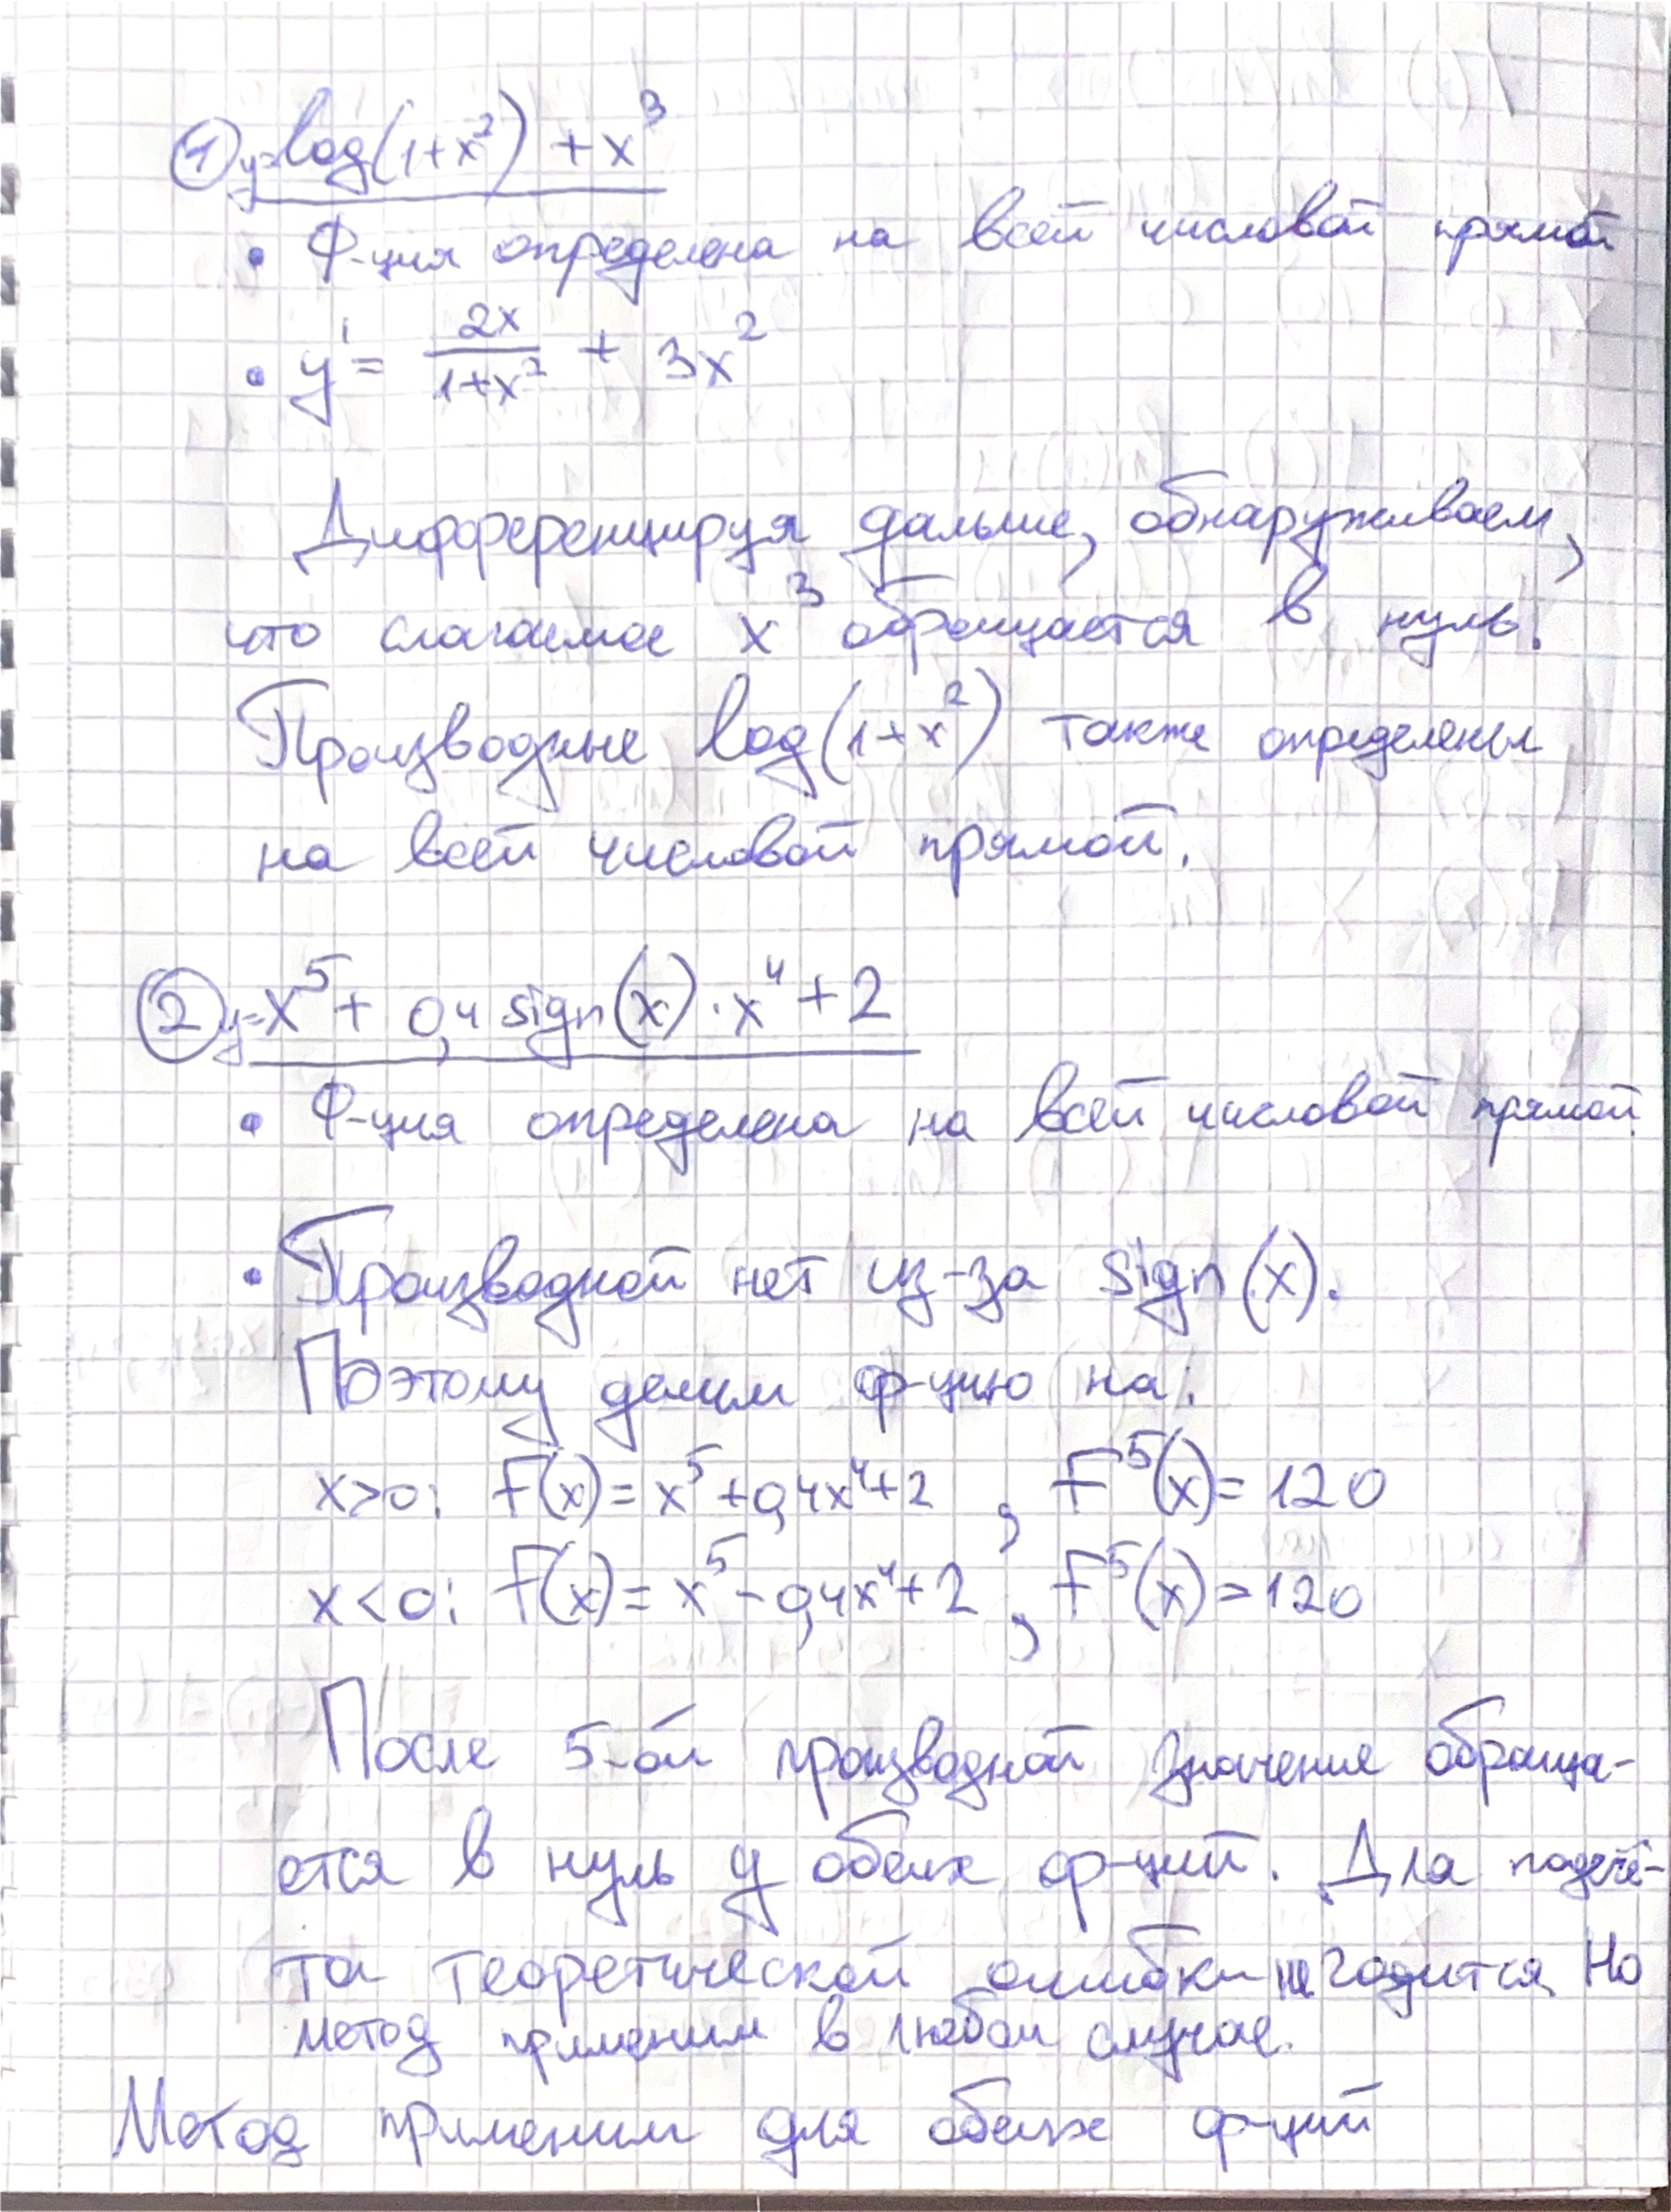
\includegraphics[width=0.9\linewidth]{../data/check.pdf}
			\caption{Проверка условий применимости для обеих функций}
			\label{fig:check}
		\end{framed}
	\end{figure}

	
	%-------- the fourth point --------
	
	\newpage
	\section{\Large \underline{Тестовый пример}}
	
	\begin{figure}[H]
		\centering
		\begin{framed}
			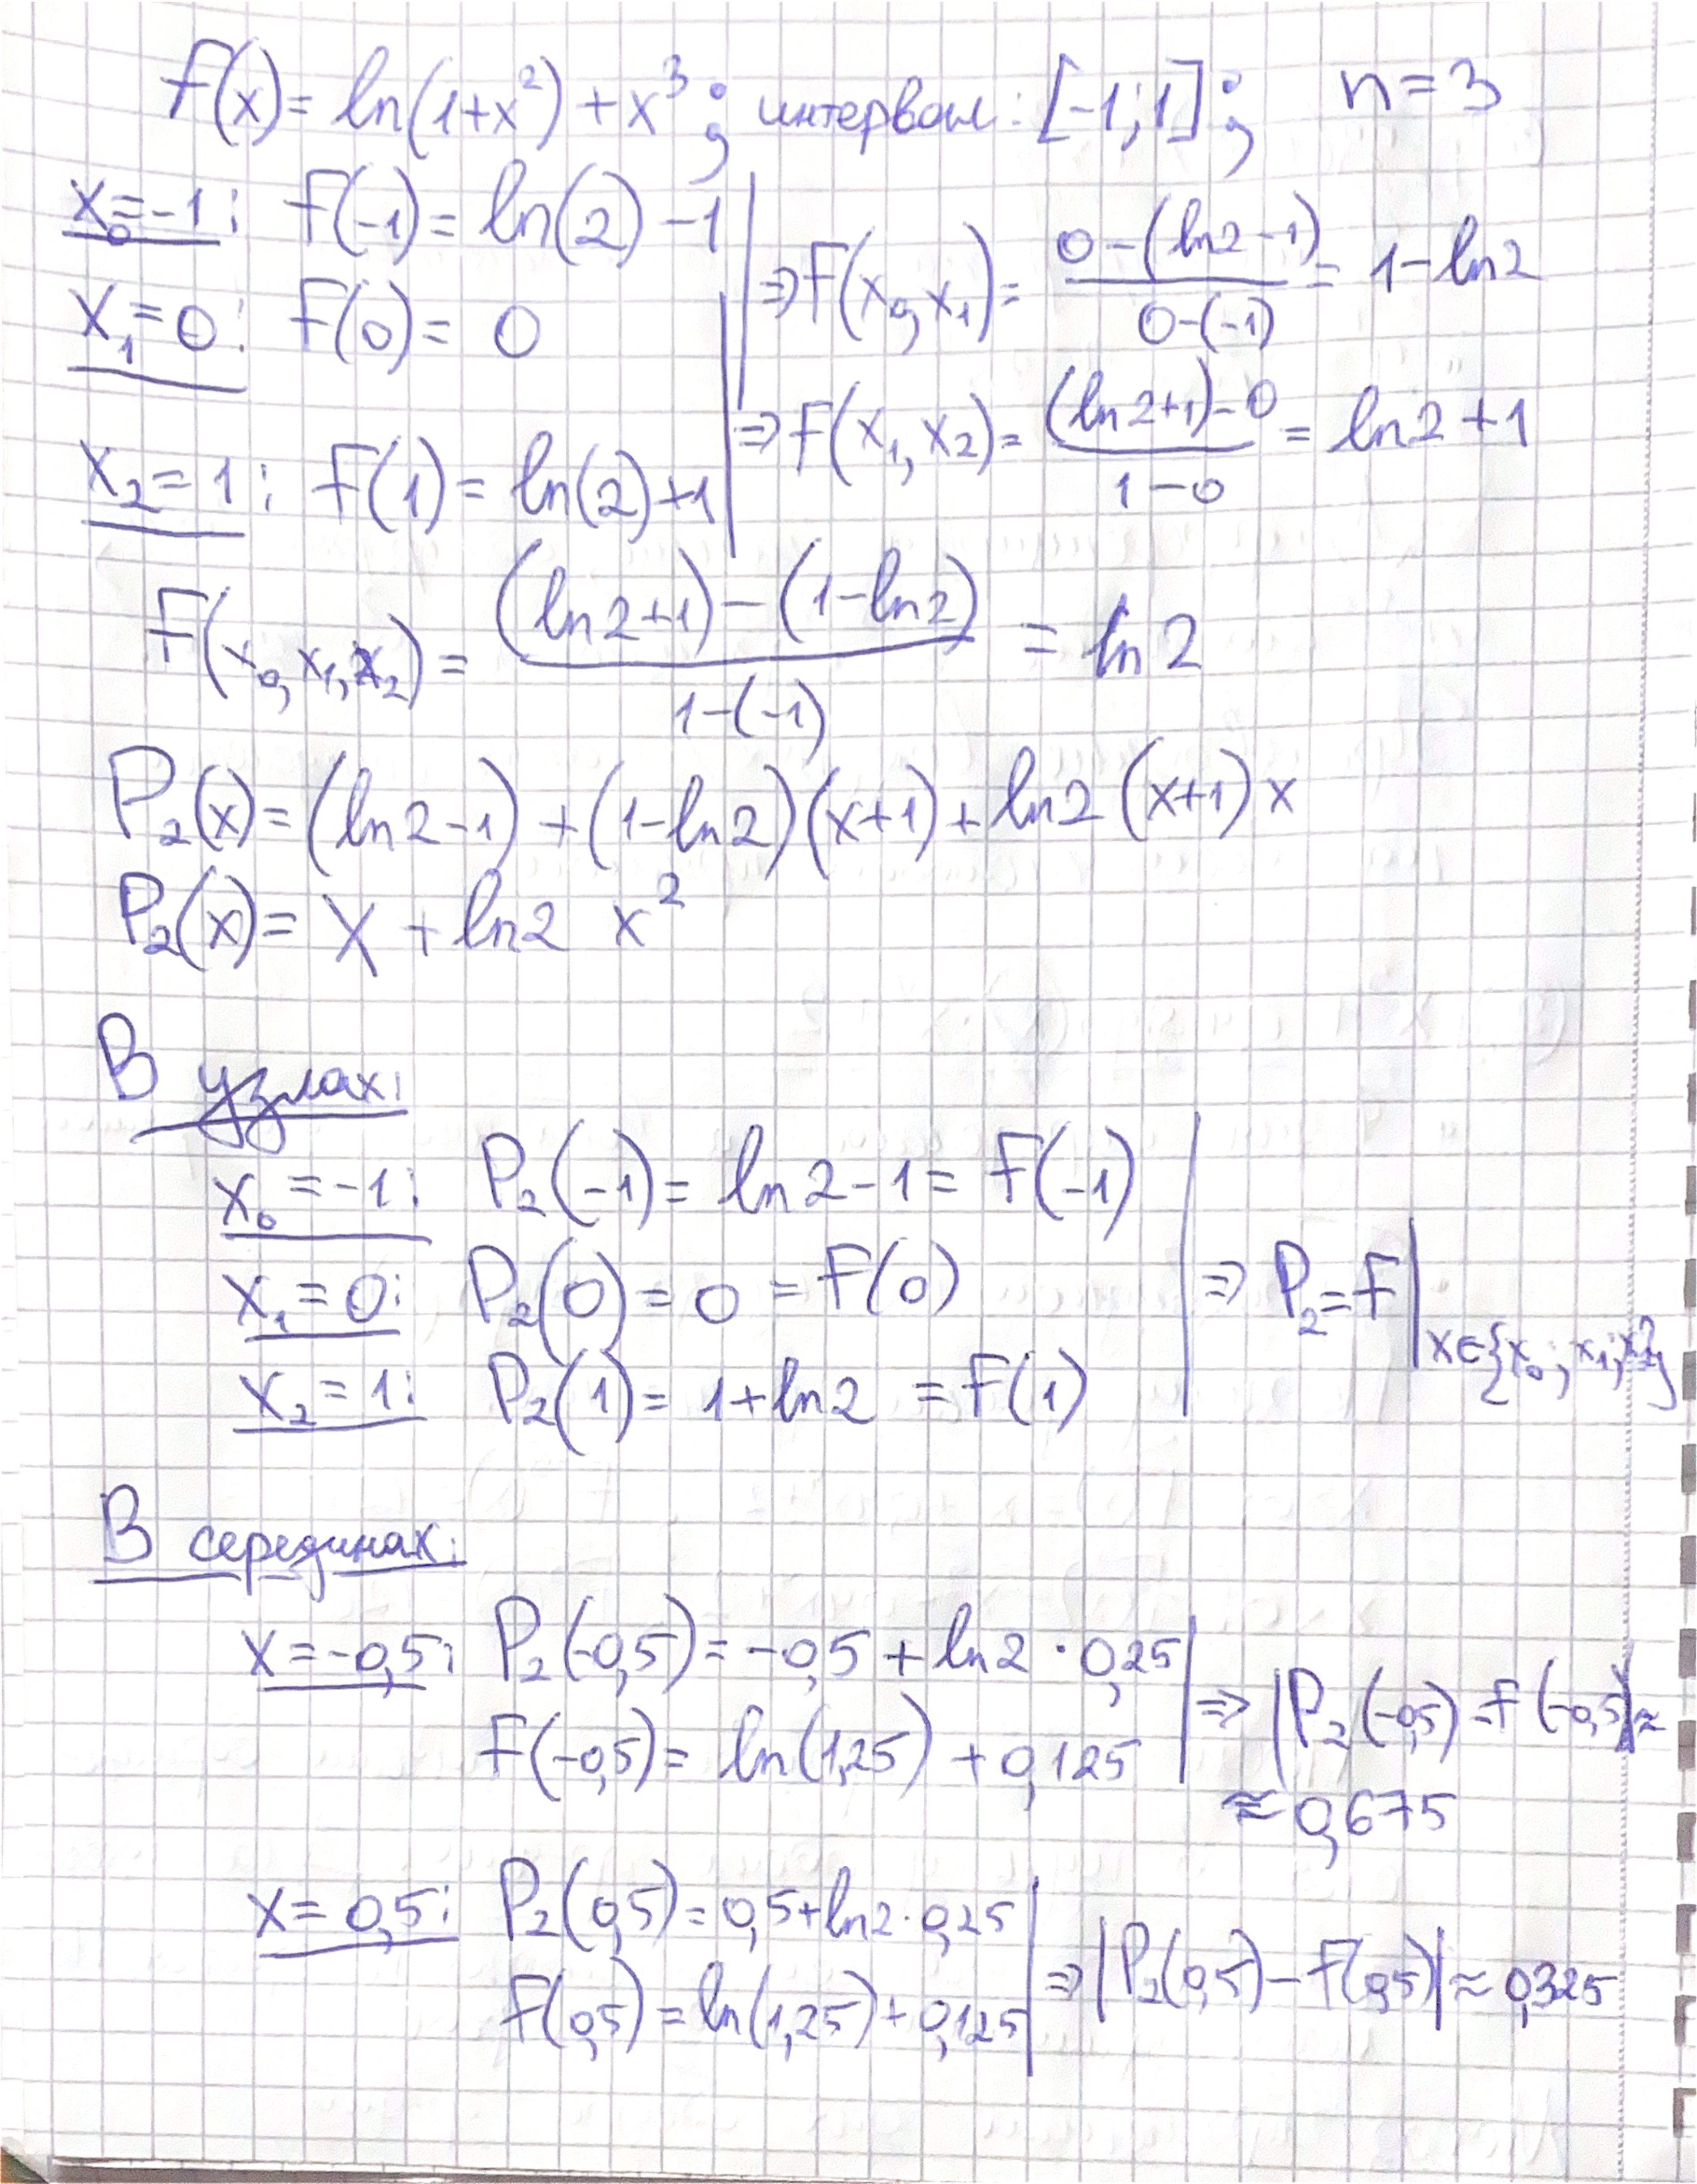
\includegraphics[width=0.9\linewidth]{../data/test.pdf}
			\caption{Тестовый пример (равномерная сетка)}
			\label{fig:test}
		\end{framed}
	\end{figure}
	
	\begin{figure}[H]
		\centering
		\begin{framed}
			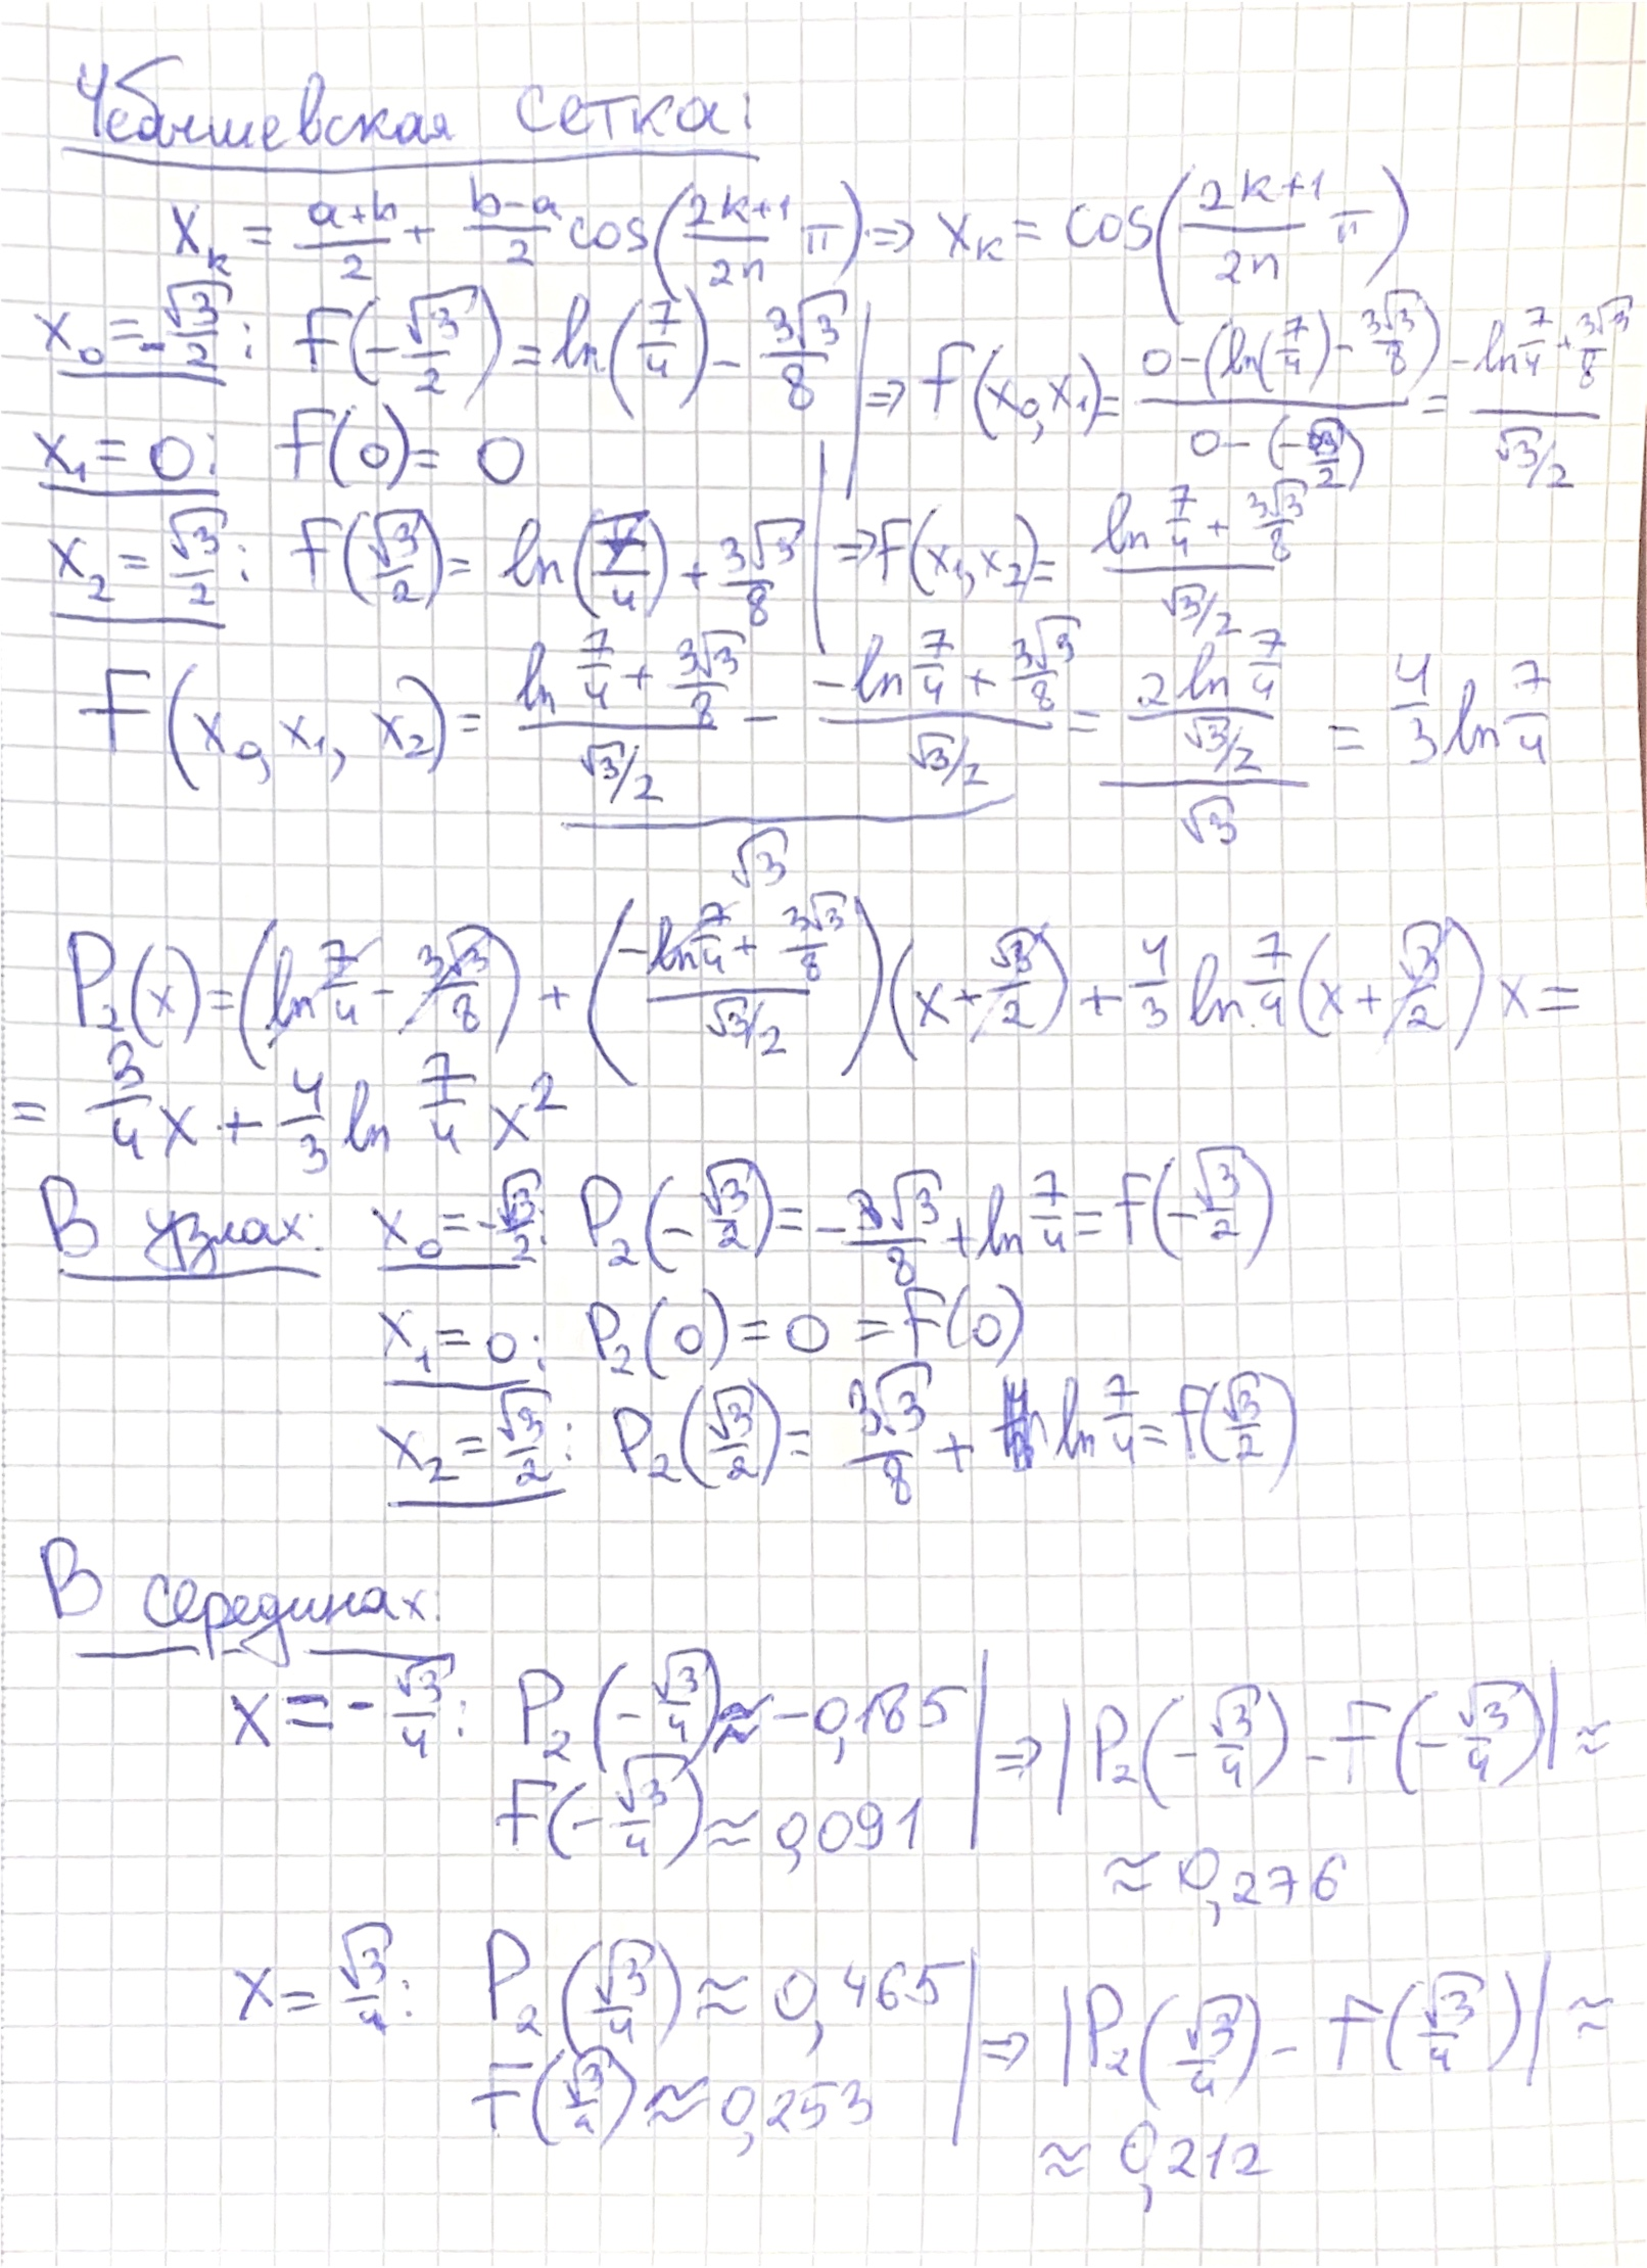
\includegraphics[width=0.9\linewidth]{../data/test_cheb.pdf}
			\caption{Тестовый пример (чебышевская сетка)}
			\label{fig:test_cheb}
		\end{framed}
	\end{figure}
	
	
	%-------- the fifth point --------
	
	\newpage
	\section{\Large \underline{Подготовка контрольных тестов}}
	
	В работе рассматриваются следующие функции:
	
	\begin{itemize}
		\item $f_1(x) = \ln(1 + x^2) + x^3$
		\item $f_2(x) = x^5 + 0.4 \cdot \mathrm{sign}(x) \cdot x^4 + 2$
	\end{itemize}
	
	Интервал интерполяции:
	\[
	[a,b] = [-2,2]
	\]
	
	Используются два типа сеток:
	\begin{itemize}
		\item равномерная сетка
		\item чебышевская сетка
	\end{itemize}
	
	Проверочная сетка содержит 10000 точек и не совпадает с узлами интерполяции. Максимальная ошибка считается на $5, ..., 100$ узлах, а полиномы строятся для $5, 7, 10$ узлов.
		
	%-------- the sixth point --------
	
	\section{\Large \underline{Модульная структура программы}}
	
	\subsection{Функции}
	\begin{itemize}
		\item \textbf{divided\_differences}\\
		функция, возвращающая разделенные разности
		\begin{table}[h]
			\begin{tabular}{|p{4cm}|p{10cm}|}
				\hline
				x & узлы \\
				\hline
				y & значения в узлах \\
				\hline
			\end{tabular}
		\end{table}
		
		\item \textbf{uniform\_grid}\\
		функция, возвращающая равномерную сетку
		\begin{table}[h]
			\begin{tabular}{|p{4cm}|p{10cm}|}
				\hline
				a & начальная точка \\
				\hline
				b & конечная точка \\
				\hline
				n & количество точек \\
				\hline
			\end{tabular}
		\end{table}
		
		\item \textbf{chebyshev\_grid}\\
		функция, возвращающая чебышевскую сетку
		\begin{table}[h]
			\begin{tabular}{|p{4cm}|p{10cm}|}
				\hline
				a & начальная точка \\
				\hline
				b & конечная точка \\
				\hline
				n & количество точек \\
				\hline
			\end{tabular}
		\end{table}
		
		\item \textbf{newton\_eval}\\
		функция, выполняющая интерполяционный метод Ньютона
		\begin{table}[H]
			\begin{tabular}{|p{4cm}|p{10cm}|}
				\hline
				x & начальная точка \\
				\hline
				coef & конечная точка \\
				\hline
				n & количество точек \\
				\hline
			\end{tabular}
		\end{table}
	\end{itemize}
	
	%-------- the eighth point --------
	
	\newpage
	\section{\Large \underline{Численный анализ решения задачи}}
	
	\begin{enumerate}[label*=\arabic*), align=left, leftmargin=*, itemindent=1.5em, listparindent=1.5em, parsep=0pt]
		\begin{figure}[H]
			\centering
			\begin{framed}
				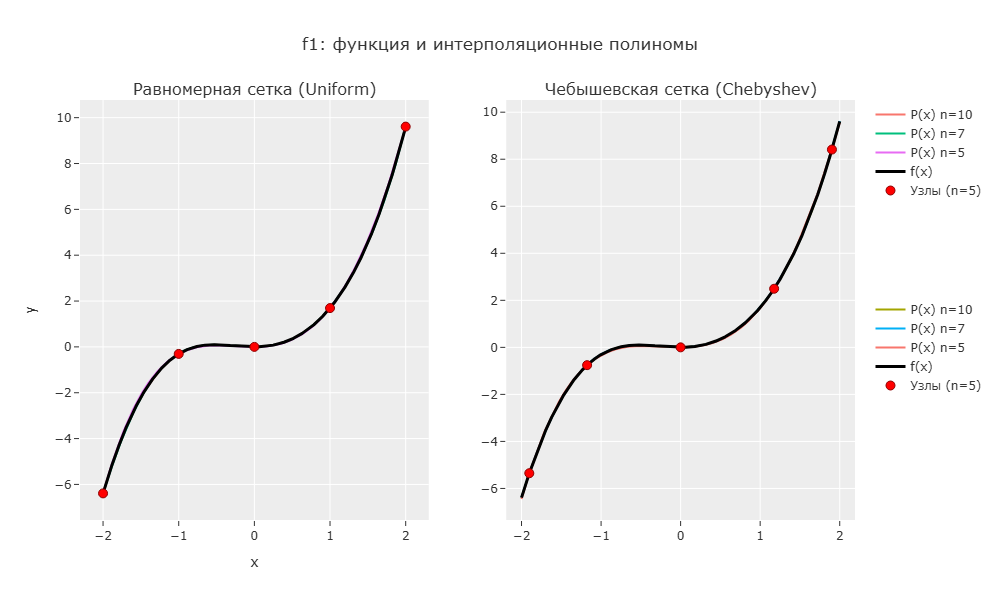
\includegraphics[width=0.9\linewidth]{../data/f1.png}
				\caption{График первой функции (сетки: слева равномерная, справа чебышевская)}
				\label{fig:f1}
			\end{framed}
		\end{figure}
		
		\begin{figure}[H]
			\centering
			\begin{framed}
				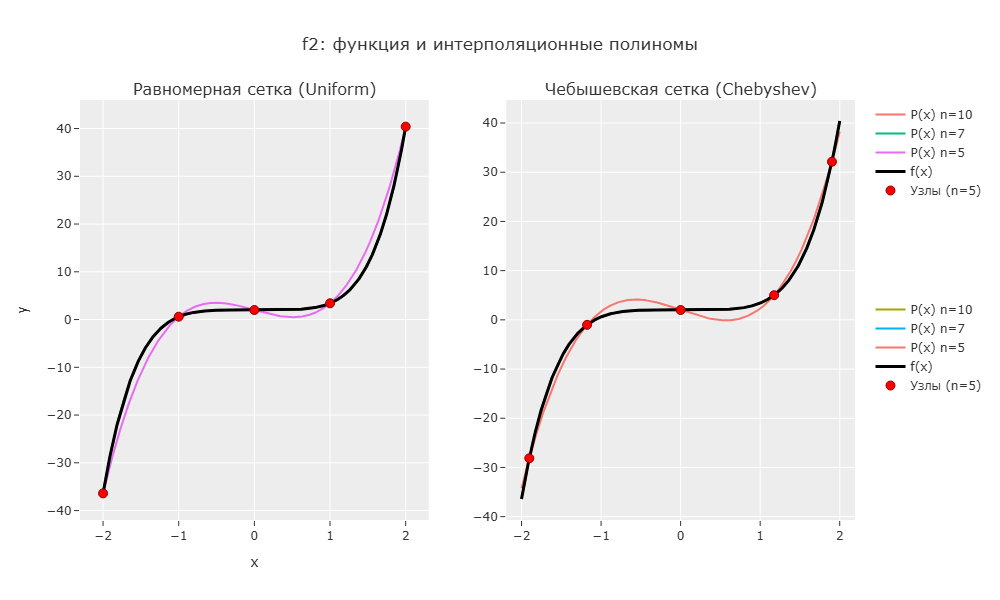
\includegraphics[width=0.9\linewidth]{../data/f2.png}
				\caption{График второй функции (сетки: слева равномерная, справа чебышевская)}
				\label{fig:f2}
			\end{framed}
		\end{figure}
		
		\begin{figure}[H]
			\centering
			\begin{framed}
				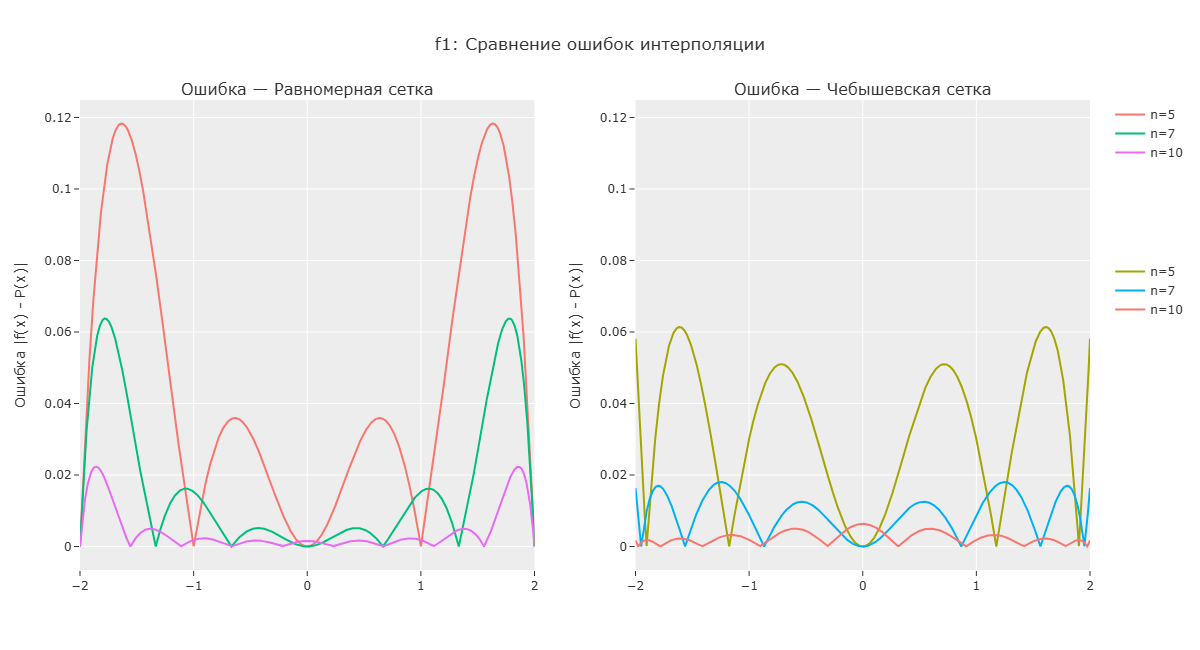
\includegraphics[width=0.9\linewidth]{../data/f1_error.png}
				\caption{График ошибки между интерполяционной зависимостью и функцией для первой функции}
				\label{fig:f1_error}
			\end{framed}
		\end{figure}
		
		\begin{figure}[H]
			\centering
			\begin{framed}
				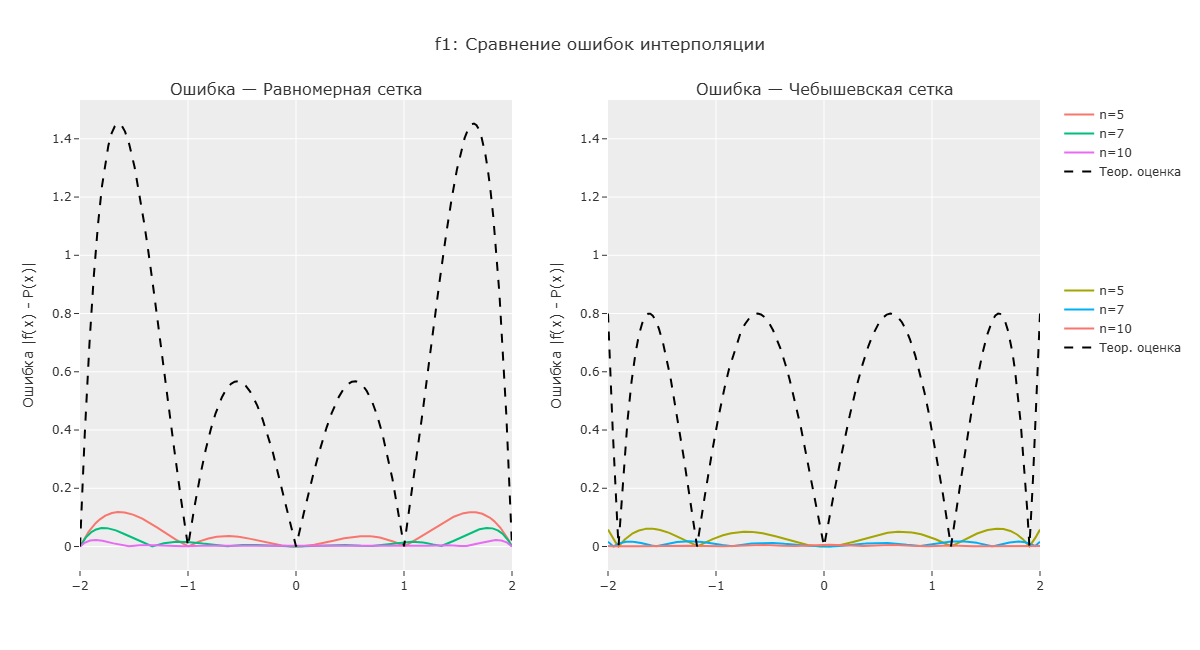
\includegraphics[width=0.9\linewidth]{../data/f1_error_with_theory.png}
				\caption{График ошибки между интерполяционной зависимостью и функцией для первой функции с теоретической ошибкой}
				\label{fig:f1_error_with_theory}
			\end{framed}
		\end{figure}
		
		\begin{figure}[H]
			\centering
			\begin{framed}
				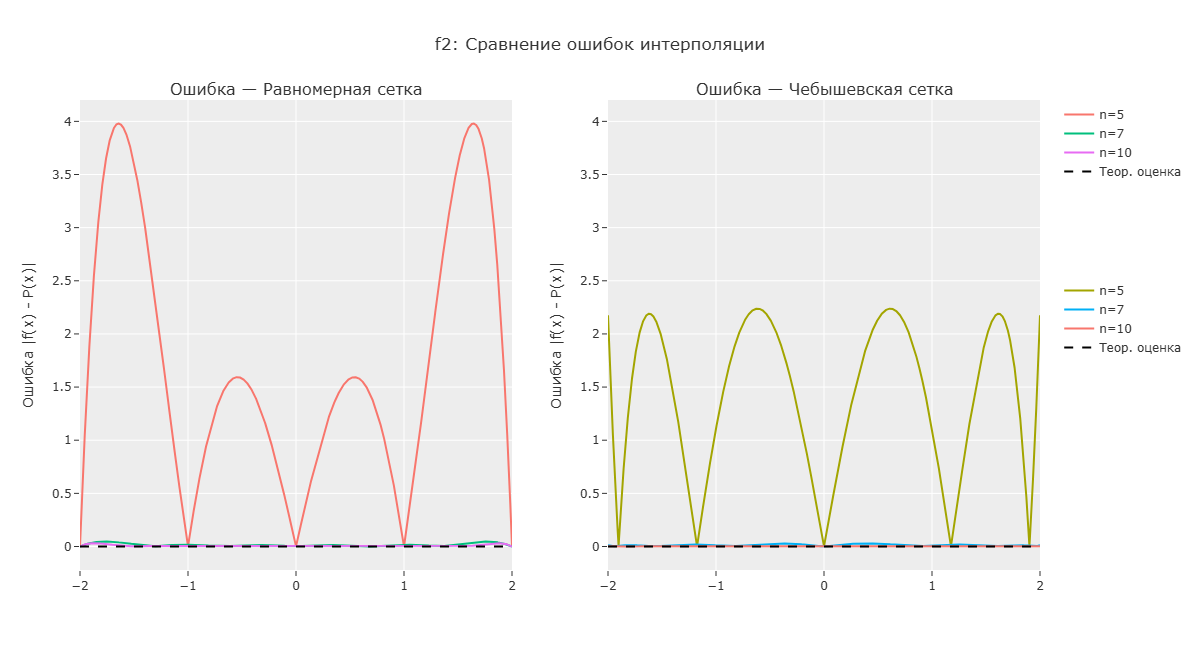
\includegraphics[width=0.9\linewidth]{../data/f2_error.png}
				\caption{График ошибки между интерполяционной зависимостью и функцией для второй функции}
				\label{fig:f2_error}
			\end{framed}
		\end{figure}
		
		\begin{figure}[H]
			\centering
			\begin{framed}
				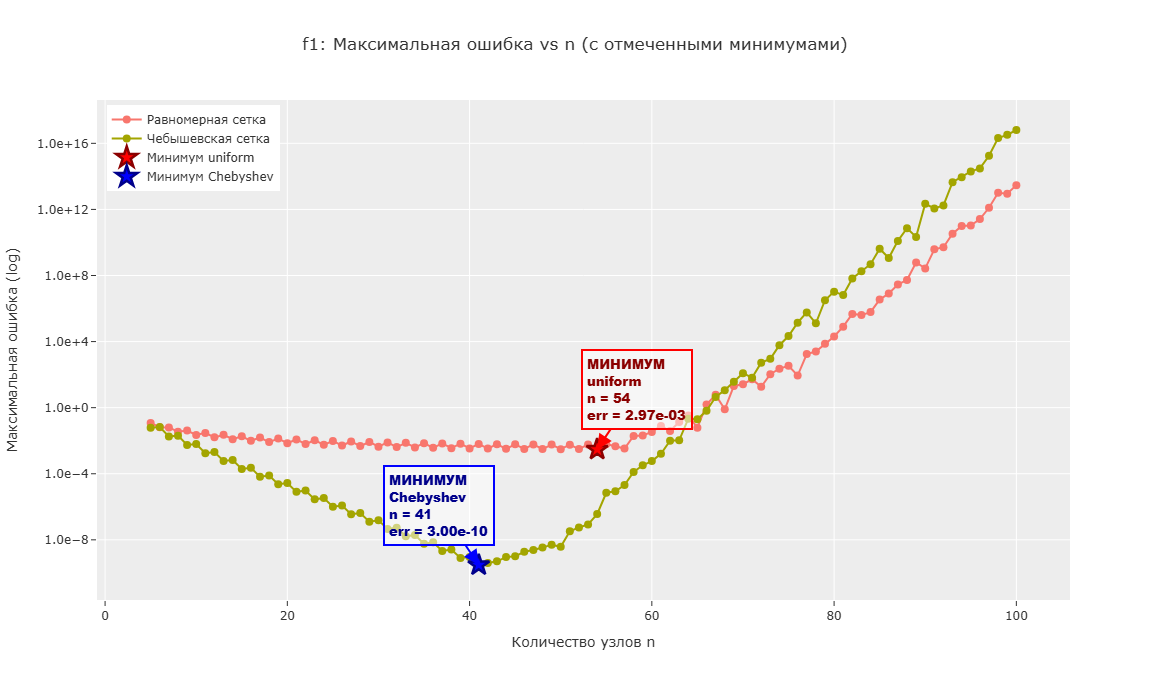
\includegraphics[width=0.9\linewidth]{../data/f1_max_error.png}
				\caption{График зависимости максимальной ошибки между интерполяцией и функцией от количества узлов для первой функции}
				\label{fig:f1_max_error}
			\end{framed}
		\end{figure}
		
		\begin{figure}[H]
			\centering
			\begin{framed}
				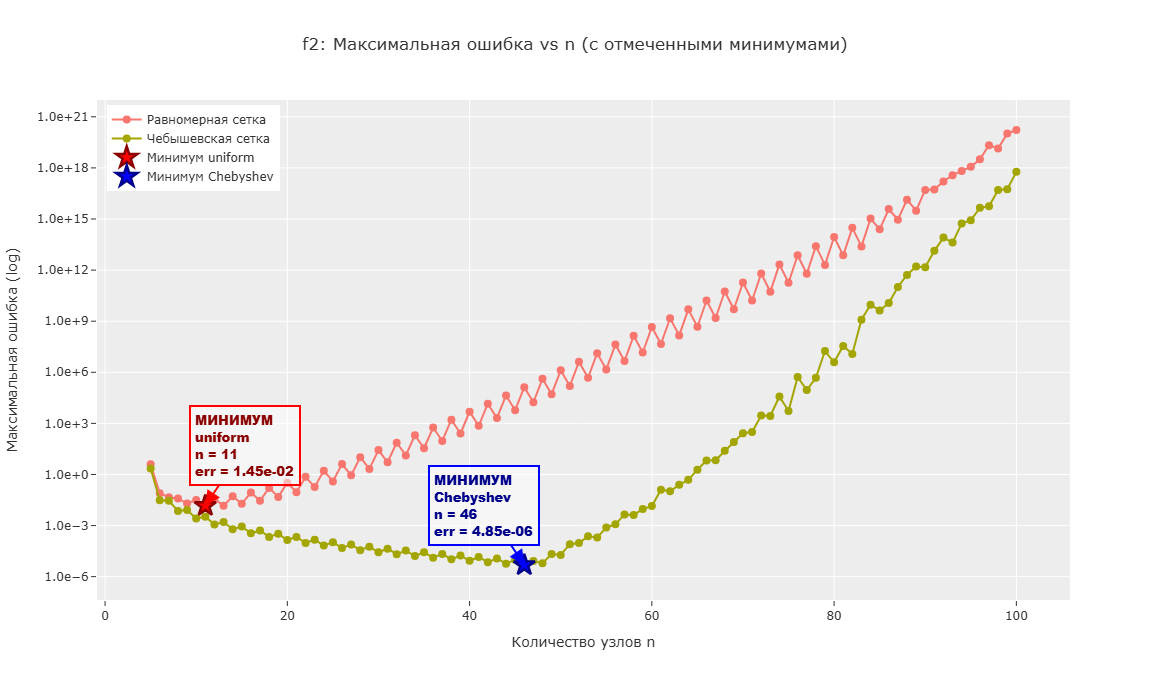
\includegraphics[width=0.9\linewidth]{../data/f2_max_error.png}
				\caption{График зависимости максимальной ошибки между интерполяцией и функцией от количества узлов для первой функции}
				\label{fig:f2_max_error}
			\end{framed}
		\end{figure}
		
		\begin{figure}[H]
			\centering
			\begin{framed}
				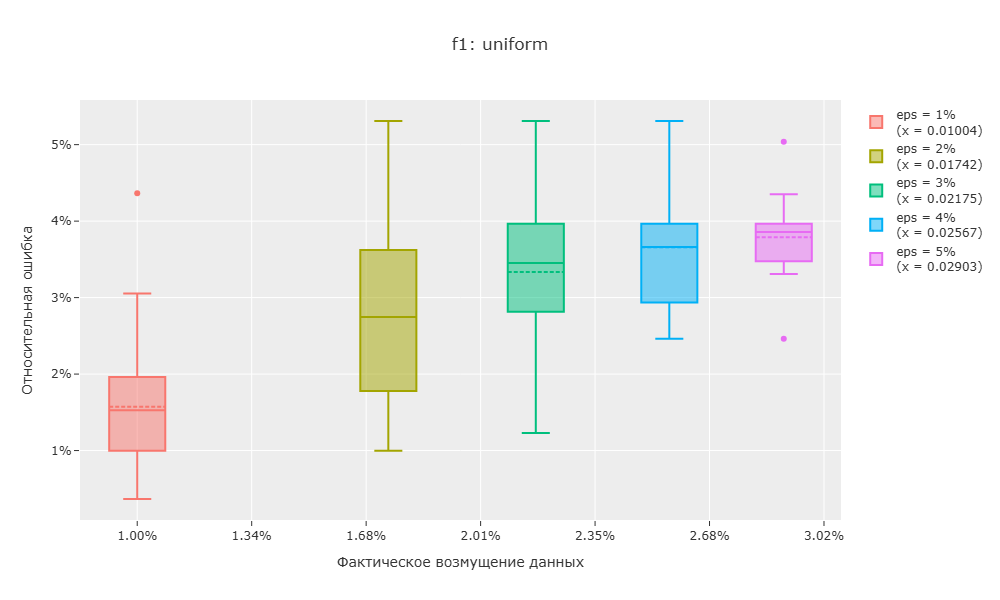
\includegraphics[width=0.9\linewidth]{../data/f1_uni_box.png}
				\caption{График зависимости ошибки от величины возмущения для первой функции (равномерная сетка)}
				\label{fig:f1_uni_box}
			\end{framed}
		\end{figure}
		
		\begin{figure}[H]
			\centering
			\begin{framed}
				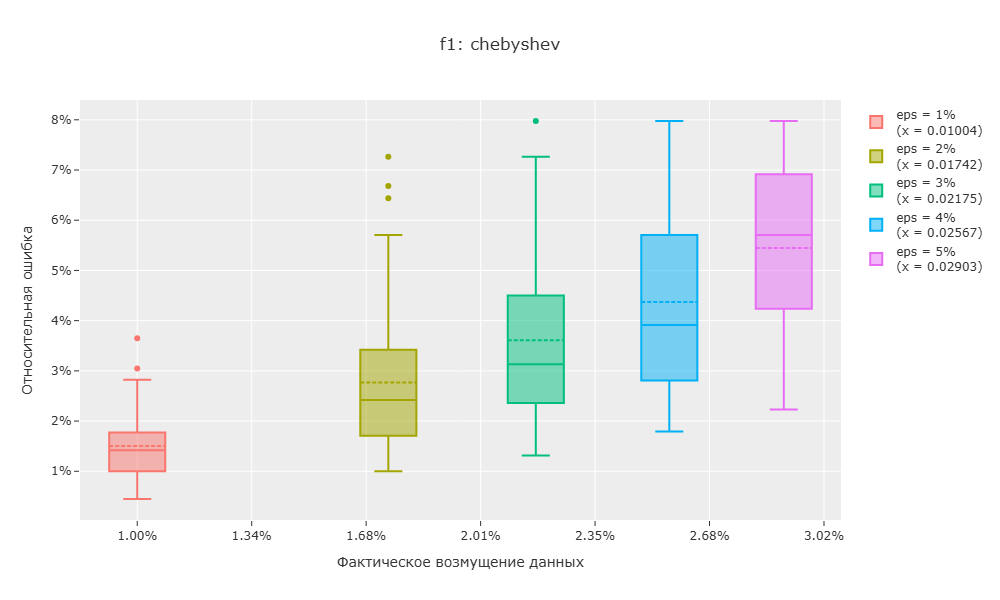
\includegraphics[width=0.9\linewidth]{../data/f1_cheb_box.png}
				\caption{График зависимости ошибки от величины возмущения для первой функции (чебышевская сетка)}
				\label{fig:f1_cheb_box}
			\end{framed}
		\end{figure}
		
		\begin{figure}[H]
			\centering
			\begin{framed}
				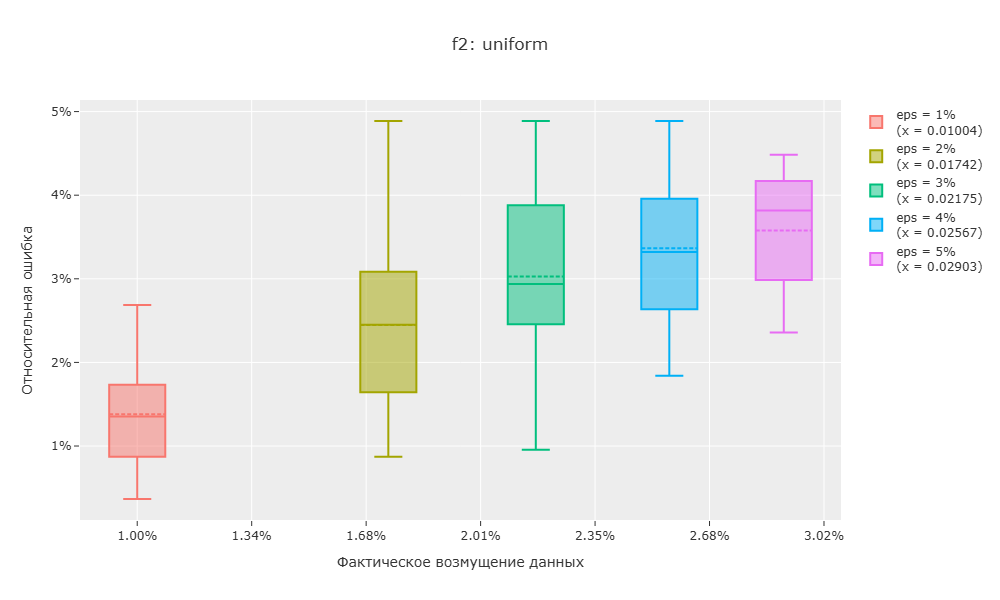
\includegraphics[width=0.9\linewidth]{../data/f2_uni_box.png}
				\caption{График зависимости ошибки от величины возмущения для второй функции (равномерная сетка)}
				\label{fig:f2_uni_box}
			\end{framed}
		\end{figure}
		
		\begin{figure}[H]
			\centering
			\begin{framed}
				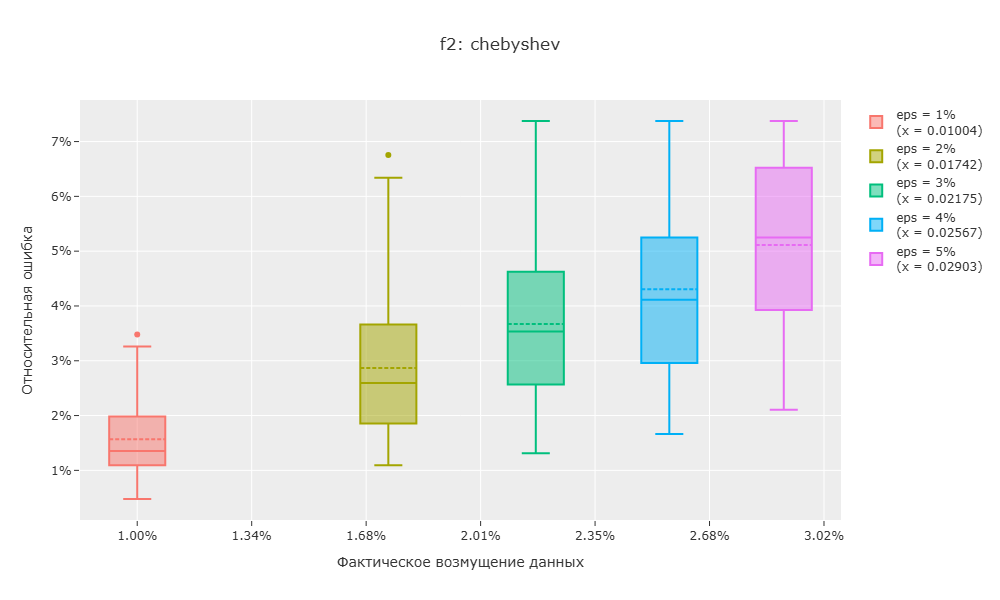
\includegraphics[width=0.9\linewidth]{../data/f2_cheb_box.png}
				\caption{График зависимости ошибки от величины возмущения для второй функции (чебышевская сетка)}
				\label{fig:f2_cheb_box}
			\end{framed}
		\end{figure}
		
		\newpage
		\item Построены изначальные полиномы для первой функции и сама функция \eqref{fig:f1}.
		
		Интерполяционный полином при малых узлах почти совпадает с исходной функцией. В связи с этим графики накладываются друг на друга. Ошибку нужно рассматривать на другом графике
		
		Построены изначальные полиномы для второй функции и сама функция \eqref{fig:f2}.
		
		Аналогично для второй функции. Хотя здесь уже и наблюдаются различия, но они минимальны чтобы делать выводы.\\
		
		\item Далее был построен график ошибок для первой функции \eqref{fig:f1_error} 
		
		Как и ожидалось, на равномерной сетке наблюдаются скачки на концах графика. Этого не наблюдать на графике чебышевской сетки, здесь ошибка имеет один и тот же характер по всему отрезку.
		
		На тот же график была добавлена теоретическая ошибка, которая была посчитана по формуле \eqref{eq:3}. Неравенство действительно выполняется, все ошибки легли под теоретическую кривую.
		
		Аналогичный график ошибок был построен для второй функции \eqref{fig:f2_error}.
		
		Здесь наблюдается та же картина с ошибкой. Однако теоретическая ошибка здесь построена неверно, поскольку эта функция не прошла условие применимости для ее подсчета.\\

		\item Рассмотрена зависимость максимальной ошибки от количества узлов сначала для первой функции \eqref{fig:f1_max_error}.
		
		При увеличении числа узлов ошибка сначала уменьшается, однако затем начинает расти. Это связано с эффектом Рунге, а также накоплением численных ошибок. Для равномерной сетки этот эффект проявляется значительно сильнее.
		
		Для равномерной сетки ошибка минимальна при 54 узлах и составляет $2.97 \cdot 10^{-3}$.
		
		Для чебышевской сетки ошибка минимальна при 41 узле и составляет $3.00 \cdot 10^{-10}$.

		Для второй функции была построена аналогичная зависимость \eqref{fig:f2_max_error}. Здесь чебышевская сетка ведет себя примерно аналогично, однако равномерная начинает расти уже на 15+ узлах.
		
		Для равномерной сетки ошибка минимальна при 11 узлах и составляет $1.45 \cdot 10^{-2}$.
		
		Для чебышевской сетки ошибка минимальна при 46 узле и составляет $4.85 \cdot 10^{-6}$.\\
		
		\item Дополнительно рассмотрены графики зависимости ошибки от величины возмущения сначала для первой функции \eqref{fig:f1_uni_box} (равномерная сетка) \eqref{fig:f1_cheb_box} (чебышевская сетка).
		
		Чебышевская сетка демонстрирует меньшую чувствительность к возмущениям данных. Это проявляется в меньшем разбросе ошибок и отсутствии выбросов. Равномерная сетка, напротив, усиливает случайные возмущения, что приводит к значительной вариативности результатов.
		
		Абсолютно такую же картину мы можем пронаблюдать и на графиках второй функции \eqref{fig:f2_uni_box} (равномерная сетка) \eqref{fig:f2_cheb_box} (чебышевская сетка).
	\end{enumerate}
	
	
	
	%-------- the ninth point --------
	
	\newpage
	\section{\Large \underline{Выводы}}
	Проделанная работа над анализом поведения метода интерполяции полиномом Ньютона позволяет сделать следующие выводы. Метод справляется со своей задачей интерполяции функции. Эффективен этот метод при малом числе узлов. Для устранения ошибок на концах отрезка следует выбирать чебышевскую сетку, которая позволяет стабилизировать ошибку и избавиться от выбросов. Немаловажно сказать о чувствительности метода к выбросам, с чем чебышевская сетка снова справляется лучше.
	
	
\end{document}